\section{Boundary conditions}
\label{sec:BCs}
%
Setting correct boundary conditions (BCs) when calculating PDEs of plasma quantities turns out to be a challenge.
In the parallel direction there will be formation of plasma sheaths between the plasma and the material which is due to the difference in mobility between the ion species and the electron species \cite{Stangeby2000book}.
This leads to a potential build-up on the material surface which affects the plasma upstream.

Unfortunately the fluid description of the plasma breaks down at the sheath as mentioned in \cite{Loizu2012a}.
This is mainly due to the fact that there will be more ions than electrons in this area and the assumption quasi-neutrality breaks down.
In other words, the fluid models are only valid up until the sheath entrance (SE), and a proper description in this area can only be accounted for with kinetic codes, solving for example the Fokker-Planck equation.
One should notice though that in reality it is hard, and maybe even impossible to tell where the bulk plasma end, and where does the sheath start.

There are mainly two challenges in setting the radial boundary conditions.
Firstly, the plasma does not usually extent all the way to the chassis of the machine, but is gradually terminated as the temperature drops and neutral dynamics takes over towards the edge.
Secondly, assuming that the plasma could extend all the way out to the chassis, the non-slip condition encountered in neutral fluid dynamics \cite{Kundu2010book} is not necessarily valid as the plasma have no way not adhere to the surface as a neutral fluid would do.

The boundaries for the cylindrical plasma consist of four parts.
In the parallel direction, we have the SE at one end.
We could in principle place a SE at the other parallel end as well, which would be OK if the plasma streamed in both direction from some point.
Instead we have chosen to model the other parallel end as a stagnation point, i.e. a point where the velocities parallel are zero.
Such a point exists if the plasma is streaming in two opposite directions, and is encountered on for example open field lines  divertor plasmas.
Radially we have the outer radial boundary condition, and an artificial inner condition which is treated in \cref{sec:innerCenter}.

The boundary conditions will be set on $n$, $u_{i,\|}$, $u_{e,\|}$ and $\Om$.
From these the boundary conditions for $j_\|$, $nu_{i,\|}$ and $\Om^D$ can be calculated in a straight forward manner.
A summary of the boundary conditions used in this thesis is found in \cref{fig:BCs}.
%
\begin{figure}[htb]
    \centering
    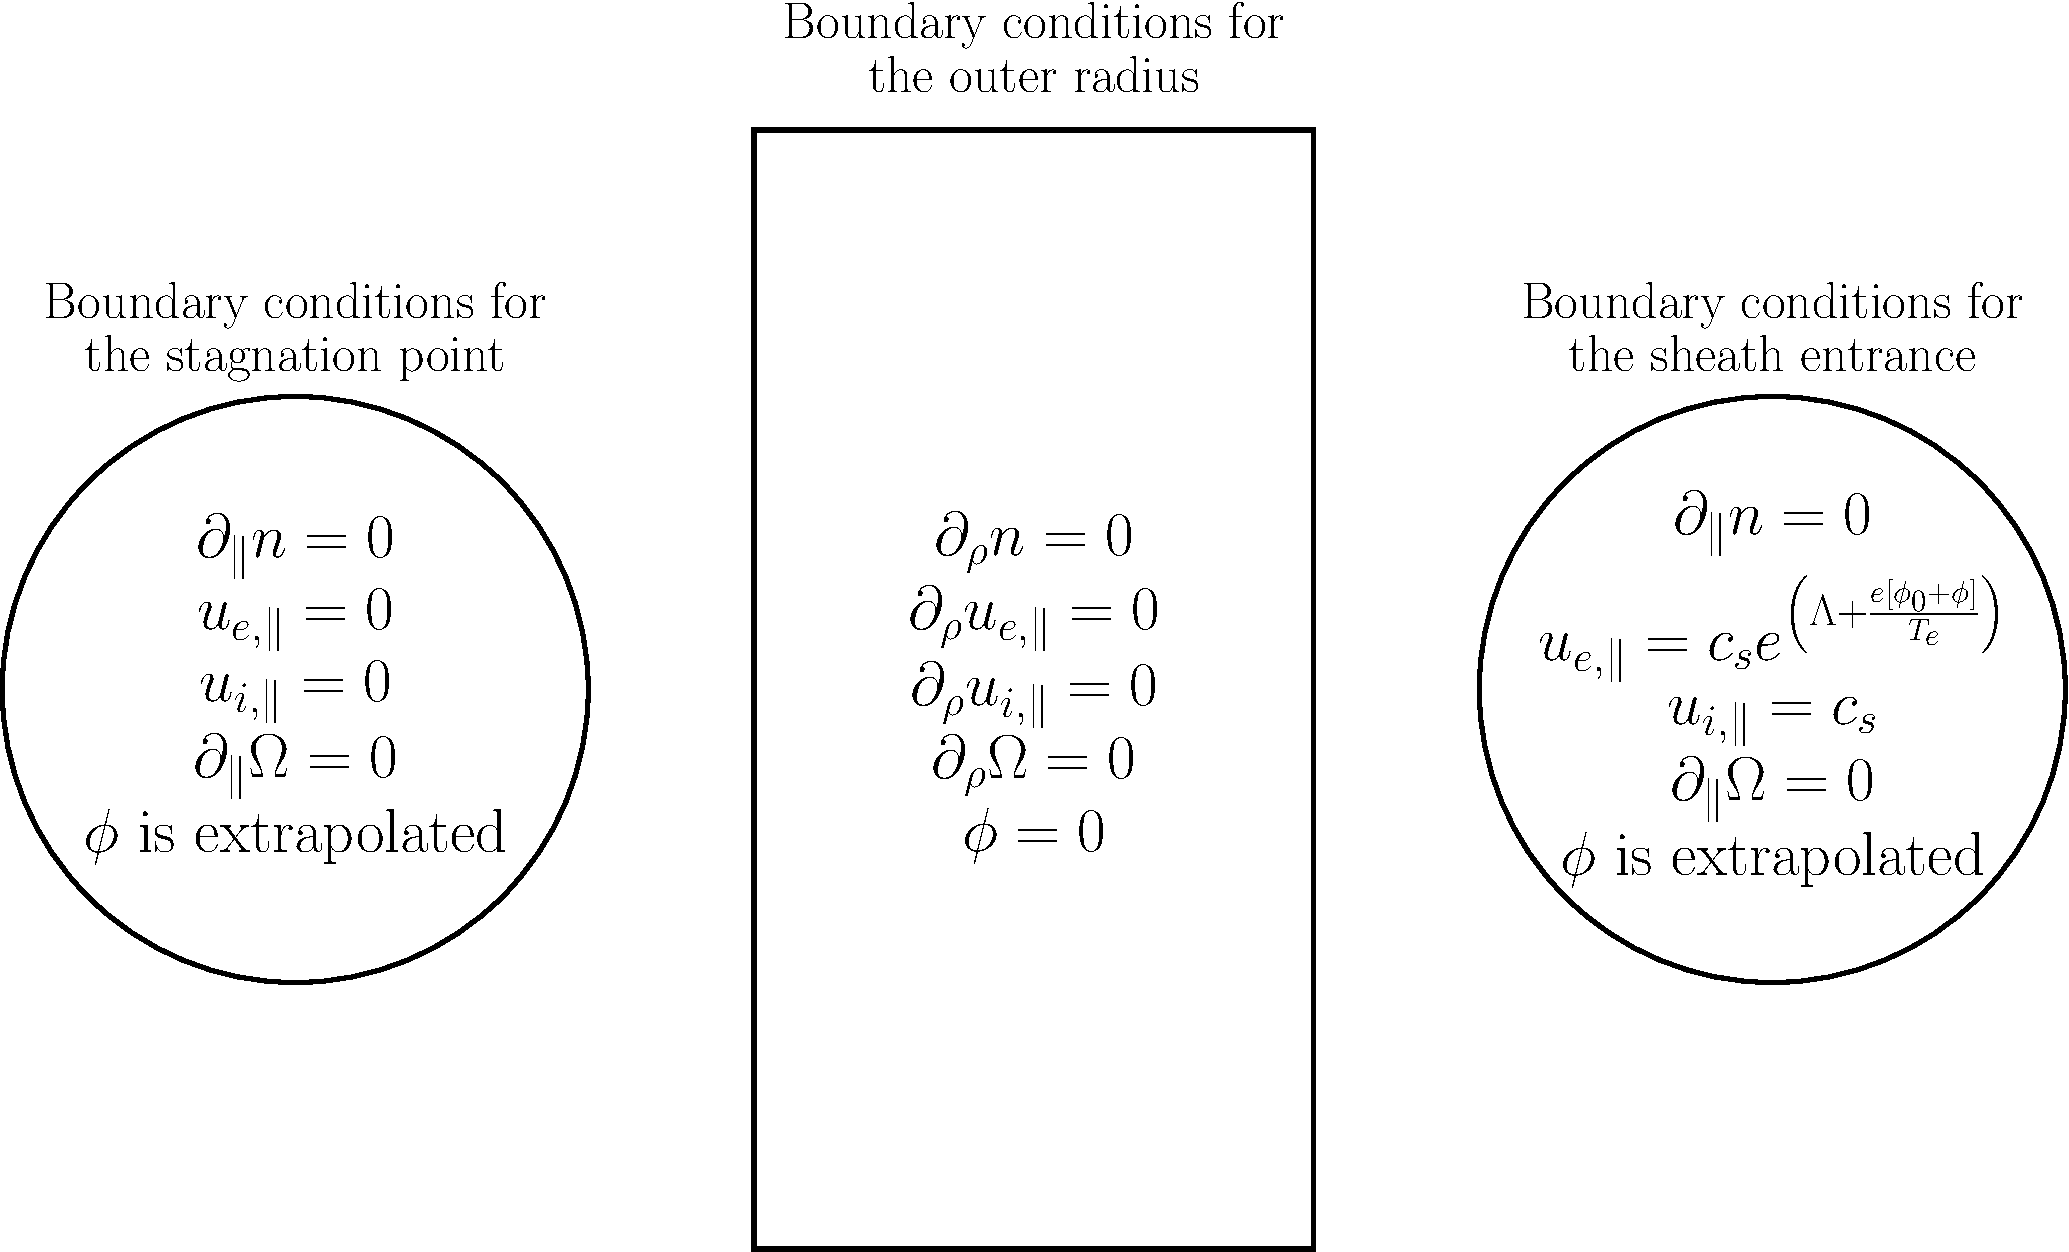
\includegraphics[width=1.0\textwidth]{fig/BCs}
    \caption{\textit{
Boundary conditions used in this thesis.
    }}
    \label{fig:BCs}
\end{figure}

\subsection{Boundary conditions at the stagnation point}
% FIXME: Add references
The boundary conditions at the opposite site of the SE in the cylinder varies from experiment to experiment (as does also the source term in the distribution function itself).
By using a stagnation point, the model does not fully reflect any experimental linear devices, but can help to shed light on some of the features found in real life experiments.
The stagnation condition acts as a kind of mirror.
To be more specific the velocities changes sign at this point, and hence must be exactly zero there.
The spinning of the plasma does not change from one side to the other across the mirror, and hence we get the following set of boundary conditions
%
\begin{align*}
    &\partial_\| n \bigg|_0    =0 &
    &u_{e,\|} \bigg|_0         =0 &
    &u_{i,\|} \bigg|_0         =0 &
    &\partial_\| \phi \bigg|_0 =0 &
    &\partial_\|\Om \bigg|_0   =0 &
\end{align*}

\subsection{Boundary conditions at the SE}
% NOTE: Consider to add calculation of sheath velocities
Following the calculations of Choudora and Bohm (see for example \cite{Stangeby2000book}), it is common practice to define the sheath entrance to be the place where ion velocity reaches the ion sound speed (that is where $u_{i,\|}=c_s$), and we will adopt this practice in this thesis.
Considering a quiescent plasma, one can calculate the equilibrium profiles which the plasma obtains in contact with materials, and use this to set the boundaries for $u_{i, \|}$ and $u_{e, \|}$ at the SE.
This is then used to calculate the boundary condition
%
\begin{align*}
    j_\|\bigg|_{L_z}=en\bigg|_{L_z}\L(u_{i, \|}\bigg|_{L_z}-u_{e, \|}\bigg|_{L_z}\R),
\end{align*}
%
where $L_z$ is the position of the SE.
One should note though, that even these boundary conditions are valid only in steady state.

\subsubsection{Ion velocity at the SE}
For the ion velocity, we have from steady state calculations defined the sheath entrance to be the point where
%
\begin{align*}
    u_{i,\|} \bigg|_{L_z} = c_s
\end{align*}
%
Normalization gives
%
\begin{align*}
    u_{i,\|} \bigg|_{L_z} = 1
\end{align*}
%

\subsubsection{Electron velocity at the SE}
%
Further, the steady state gives the following condition on the parallel electron velocity
%
\begin{align*}
    u_{e,\|} \bigg|_{L_z} = c_s \exp\L(\Lambda - \frac{e[\phi_0 + \phi]}{T_e}\R),
\end{align*}
%
where $\phi_0$ is an arbitrary potential and $\Lambda=\ln\L(\sqrt{\frac{\mu}{2\pi}}\R)$.
In this thesis, we set $\phi_0=\Lambda T_e/e$, so that $\phi=0$ for ambipolar flow%
%
\footnote{We do this as we have observed that the inversion algorithm for $\phi$ mentioned in \cref{app:lapInv} is more numerically stable}%
%
.
Normalization gives
%
\begin{align*}
    u_{e,\|} \bigg|_{L_z} = \exp\L(\Lambda - \phi\R)
\end{align*}
%

\subsubsection{Density BC at the SE}
%
% NOTE: Tried
%   1. From steady state electron continuity
%      This means that n cannot change at the boundary
%   2. Neumann = 0
%      Could be that this it has a gradient
%      Problem that Neumann both at the SE and non-SE site
% NOTE: Idea
%   1. Could try robin BC at non-SE site
%
Although the "standard" calculation for the sheath gives us conditions for setting the velocities in steady state, non such conditions exists for the density.
Instead, one would have to rely on other arguments.
In \cite{Loizu2012a}, Loizu et al.  presents a boundary condition for the density in a field line geometry, where the field lines are allowed to be tilted with respect to the end-plate.
For a field line geometry where the field lines are perpendicular to the end-plate (which is the case in this thesis), the boundary condition reduces to
%
\begin{align*}
    \L. \partial_\| n \R|_{L_z}&= -\L.\frac{n}{c_s}\partial_\| u_{i.\|}\R|_{L_z}\\
    \note{$\L. u_{i.\|}\R|_{L_z} = c_s$}
    \L.u_{i.\|} \partial_\| n \R|_{L_z}&= -\L.n \partial_\| u_{i.\|}\R|_{L_z}\\
    \L.u_{i.\|} \partial_\| n \R|_{L_z}+\L.n \partial_\| u_{i.\|}\R|_{L_z}&= 0\\
    \L.\partial_\|\L(u_{i.\|}  n \R)\R|_{L_z}&= 0\\
    \L.\ve{b}\cdot\grad\L(u_{i.\|}  n \R)\R|_{L_z}&= 0
    \note{$\partial_i \ve{b} = 0$}
    \\
    \L.\div\L(\ve{b}u_{i,\|}  n \R)\R|_{L_z}&= 0\\
    \L.\div\L(\ve{u}_{i,\|}  n \R)\R|_{L_z}&= 0\\
    \L.\L(\grad_\perp + \grad_\|\R)\cdot\L(\ve{u}_{i,\|} n \R)\R|_{L_z}&= 0\\
    \L.\grad_\|\cdot\L(\ve{u}_{i,\|} n \R)\R|_{L_z}&= 0
    \note{$\grad_\| \cdot \ve{u}_{i,\perp} = 0$}
    \\
    \L.\grad_\|\cdot\L(\ve{u}_{i} n \R)\R|_{L_z}&= 0
    \note{Continuity equation}
    \\
    \L.- \partial_tn \R|_{L_z}- \L.\grad_\perp\cdot\L(\ve{u}_{i} n \R)\R|_{L_z} + S_{i,n}&= 0\\
    \L.\partial_tn \R|_{L_z}&=  - \L.\grad_\perp\cdot\L(\ve{u}_{i} n \R)\R|_{L_z} + S_{i,n}
    \numberthis
    \label{eq:nBC}
\end{align*}
%
In other words, it says that the only change in the density (appart from the source) jjjjjjjjjjjjjjjjjat the SE can come from perpendicular outflux.
Another way to look at it is to consider
%
\begin{align*}
    \L.\L[\inde{\partial_\|\L(u_{i.\|}  n \R)}{z}\R]\R|_{L_z}&= 0\\
    \L.u_{i.\|}  n \R|_{L_z}&= C
\end{align*}
%
which means that the flux through the SE is constant in time, which may be a too big constraint on the system.

One alternative is to set
%
\begin{align*}
    \L. \partial_\| n \R|_{L_z} &= 0
\end{align*}
%
If we follow the derivation of \cref{eq:nBC} and use the ion continuity equation, this can be written as
%
\begin{align*}
    \L.- \partial_tn \R|_{L_z}- \L.\grad_\perp\cdot\L(\ve{u}_{i} n \R)\R|_{L_z}
    -\L.n \partial_\| u_{i.\|}\R|_{L_z} + S_{i,n}
    &= 0\\
    \L.\partial_tn \R|_{L_z}&=  - \L.\grad_\perp\cdot\L(\ve{u}_{i} n \R)\R|_{L_z}-
    \L.n \partial_\| u_{i.\|}\R|_{L_z} + S_{i,n}
\end{align*}
%
which means that the flux through the SE is no longer fixed.
One should note though that this boundary condition will try to enforce a zero gradient on $n$ at the SE, which migth be unphysical.
Also one should note that if one has a Neumann condition in both ends of the machine, the PDE is formally ill-posed, and the solutions found are unique only up to some constant.
When numerically solving the system the solution found will be specified by the initial condition.
Although it is important to be aware of, it is not believed to change the physical behavior of the system as the dynamics are driven by its source and its sinks.

A third approach, which does not have the same problem, is to let the density be completely free at the sheath entrance and instead fix the value and the gradient at the stagnation point (where the velocities are $0$) using a Cauchy boundary condition (not to be confused with a Robin or "mixed" boundary condition).
This kind of boundary condition specifies the parallel dynamics fully.
The derivatives of $n$ at the last physical point before the SE can then be calculated numerically either by a one-sided stencil, or by extrapolating the solution to a ghost point%
%
\footnote{A ghost point is a point not belonging to the physical domain, but a helper point which makes it possible to use a centered scheme when evaluating a grid point closest to the physical boundary of the domain.}
%
and use this is an \emph{artificial boundary condition} \cite{Leveque2007book}.

A final possibility is to let the derived equation for the evolution of the density be valid at the boundary.

In the scope of this thesis the $\L. \partial_\| n \R|_{L_z} = 0$ boundary condition has been choosen.
% FIXME: Remove the comment below if Cauchy is not considered
% In the scope of this thesis the differences between $\L. \partial_\| n \R|_{L_z} = 0$ and the Cauchy BC has been investigated.

\subsubsection{Potential BC at the SE}
%
% NOTE: Tried
%   1. Fixed value
%      Bad idea, as difference in parallel velocities are not regulated by the
%      potential
%   2. Neumann 0
%      Bad idea as this may make an artificial constraint on the system
The potential in our equations are not being evolved in time directly, but is calculated by inverting either $\Om$ or $\Om^D$ for each drift plane (that is for each perpendicular plane).
This inversion takes into account the outer radial boundary condition in $\phi$.
This outer radial boundary condition can be set from the material properties of the wall.
On the other hand, we do not have any physical material constraint at the SE.
The only thing we impose it that $\phi$ on the plate very close to the SE is set to an arbitrary constant.
 It is not clear how this is reflected at the SE in a non-steady state plasma.

However, parallel derivatives of the potential is being taken in our set of equations.
In order to calculate the parallel derivative of $\phi$ in the last point before the SE, we need either to make a one sided stencil for this very point (as the value of the boundary, and thereby the value of the ghost point is unknown), or we can extrapolate the value of $\phi$ to the ghost point (as we anyway assume that $\phi$ is a smooth function in order to discretize the differential operators working on $\phi$).
The latter has been chosen in the current implementation, with the polynomial given in \cref{sec:extrapolGhost}.

\subsubsection{Vorticity BC at the SE}
% NOTE: Tried
%   1. Neumann = 0
%      Could be that this it has a gradient
%      Problem that Neumann both at the SE and non-SE site
% IDEA:
%   1. Should be 0, as the wall is slowing down? Maybe not as not necessarily
%      have a non-slip BC on the wall
As with $\phi$, the sheath boundary condition sets no restrain on the vorticity at the SE.
However, as $\Om$ is a variable being solved in time, a boundary condition is needed in order to fully specify the system.
In the current implementation $\L. \partial_\| \Om \R|_{L_z} = 0$ has been chosen.
Note that this may not be a particularly good boundary condition as it physically means that there can be no parallel shear in the perpendicular spinning at the SE.

\subsection{Outer radial boundary conditions}
\label{sec:outerBC}
%
The radial boundary conditions can in principle determine the results of the experiments entirely.
This have been seen in experiments on for example the Mirabelle machine \cite{Schroder2001}.
However, to correctly asset the physics, one would have to take into account the neutral interaction and the material properties of the wall.
We will therefore in this thesis focus on a much simplified approximation of the radial boundary conditions.
In fact we will let the radial boundary condition be approximately where the neutrals are dominating, and thus dampening out the plasma dynamics.

\subsubsection{Density BC at outer radius}
As the density will go toward $0$ as we are approaching the wall, we could set
%
\begin{align*}
    n \bigg|_{L_\rho} = C,
\end{align*}
%
where $C$ is a small constant.
Setting this too small, however can give rise to numerical problems due to loss of precision.

In this thesis, another approach has been used.
As the density profile is approximately Gaussian, the profile will be relative flat towards the radial edge.
We therefore set
%
\begin{align*}
    \partial_\| n \bigg|_{L_\rho} = 0
\end{align*}
%
Note however that this can be too restrictive if coherent structures such as "blobs"
% FIXME: Add blob reference, krashenenikov and grulke naulin
are reaching the domain boundary.

\subsubsection{Velocity BCs at outer radius}
% Not really physically explained
% If we let u_|_ =\= 0 we have no physical explanation why this should be 0
%
The parallel velocities are not constrained by any forces at the radial edge, and can thus take any value.
In this thesis we set
%
\begin{align*}
    \partial_\| u_{e,\|} \bigg|_{L_\rho} = \partial_\| u_{i,\|} \bigg|_{L_\rho} = 0
\end{align*}
%
although there in principle are no physical reason for why this should be.

\subsubsection{Potential BC at outer radius}
%
There are no sheath where the magnetic field lines are perpendicular to the material.
Thus, if we assume that the chassis is an ideal conductor, the potential there should be at the floating potential if we exclude finite Larmor radius (FLR) effects.
For that reason we have that
%
\begin{align*}
    \phi \bigg|_{L_\rho} = 0
\end{align*}
%
As the ion Larmor radius is larger than the electron Larmor radius, more ions than electron would be lost radially initially if FLR effect were included.
This would result in a small potential difference which would increase the poloidal $\ve{E}\times\ve{B}$ drift.

\subsubsection{Vorticity velocity BC at outer radius}
%
% NOTE: Tried
%       1. Om = 0
%       This will give rise to a boundary layer which will try to oppose the
%       eventual solid body rotation in the center
% NOTE: The boundary here is set from either the non-slip or the free-slip
%       condition of v_theta
%
As stated in the introduction of \cref{sec:BCs}, there exists no analogue to the no-slip condition in plasmas.
In other words, there is nothing which constrains the poloidal flow at the material surface.
As a consequence, there will be nothing constraining the poloidal flow at the position where the plasma terminates (where neutrals are starting to dominate) radially.
One could assume that
%
\begin{align*}
    \Om \bigg|_{L_\rho} = 0,
\end{align*}
%
which is set in this thesis, although no physical explanation for this is given.

\subsection{Inner radial boundary conditions}
\label{sec:BCInnerRho}
%
Physically, there are no boundary condition around the central axis of a cylinder.
However, we need some artificial boundary conditions around this area as our domains covers $\rho \in \; ]0, L_\rho[$ (where $L_\rho$ is the radius of the system) and we are using a finite difference (FD) scheme to calculate radial derivatives.
As this is not related to the physics of the problem, the discussion is given in \cref{sec:innerCenter}.
